% Uncomment this to make slides with overlays:
%\documentclass[slides]{beamer}

% Uncomment these (but comment the above \documentclass line) to make handouts:
\documentclass[handout]{beamer}

% Uncomment these to have more than one slide per page
\usepackage{pgfpages}
\pgfpagesuselayout{2 on 1}[border shrink=5mm]
\pgfpageslogicalpageoptions{1}{border code=\pgfusepath{stroke}}
\pgfpageslogicalpageoptions{2}{border code=\pgfusepath{stroke}}

\usepackage[]{graphicx, color, hyperref}

\mode<presentation>
{
	%\usetheme[secheader]{Boadilla}
	%\usecolortheme[rgb={.835, .102,.169}]{structure}  
	\usetheme[width= 0cm]{Goettingen}
	%\setbeamercovered{transparent}
}
\setbeamertemplate{navigation symbols}{}
\setbeamertemplate{footline}[frame number]

\definecolor{blue2}{rgb}{0.278,0.278,0.729} 
\newcommand{\blue}[1]{\textcolor{blue2}{#1}}
\newcommand{\white}[1]{\textcolor{white}{#1}}
\newcommand{\red}[1]{\textcolor{red}{#1}}
\newcommand{\xbar}{\overline{x}}
\newcommand{\ybar}{\overline{y}}
\newcommand{\phat}{\widehat{p}}
\newcommand{\prob}{\mbox{Pr}}
\newcommand{\E}{\mathbb{E}}
\newcommand{\Var}{\mbox{Var}}
\newcommand{\cp}{\oplus}
\newcommand{\cm}{\circleddash}

\title{Lecture 15: Hypothesis Testing Part II}
\author{Chapter 4.3}
\date{}


\begin{document}
%------------------------------------------------------------------------------
\begin{frame}
\titlepage
\end{frame}
%------------------------------------------------------------------------------


%------------------------------------------------------------------------------
\begin{frame}[fragile]
\frametitle{Goals for Today}

\begin{itemize}
\item Define significance level
\item Tie-in p-Values with sampling distributions
\item Example
\end{itemize}

\end{frame}
%------------------------------------------------------------------------------


%-------------------------------------------------------------------------------
\begin{frame}
\frametitle{Type I Errors:  US Criminal Justice System}
Defendants must be ``guilty beyond a reasonable doubt'': better to let a guilty person go free, than put an innocent person in jail.  

\pause\vskip 0.25cm

\begin{itemize}
\item $H_0$: the defendant is innocent
\item $H_A$: the defendant is guilty
\end{itemize}
\pause thus ``rejecting $H_0$'' is a guilty verdict $\Rightarrow$ putting them in jail

\vskip 0.25cm

\pause In this case:
\begin{itemize}
\item Type I error = jailing an innocent person (worse)
\item Type II error = letting a guilty person go free.  
\end{itemize}
\end{frame}
%-------------------------------------------------------------------------------


%-------------------------------------------------------------------------------
\begin{frame}
\frametitle{Type II Errors: Airport Screening}
An example of where Type II errors are more serious:  \blue{airport screening}. 
\pause \begin{eqnarray*}
H_0: && \mbox{passenger X does not have a weapon}\\
H_A: && \mbox{passenger X has a weapon}
\end{eqnarray*}
\pause Failing to reject $H_0$ when $H_A$ is true is not ``patting down'' passenger X when they have a weapon.
\vskip 0.25cm
\pause Hence the long lines at airport security.  
\end{frame}
%-------------------------------------------------------------------------------


%-------------------------------------------------------------------------------
\begin{frame}
\frametitle{Significance Level}

%
% Comment this
%
%The philosophy of hypothesis testing is to not reject $H_0$ unless we have strong evidence.  i.e. control Type I errors.
%
%\pause \vspace{0.5cm}
%
%Example: when $H_0$ is true, if we do not want to incorrectly reject $H_0$ more than 5\% of the time, set $\alpha = 0.05 = 5\%$. $\alpha$ is the \blue{significance level}.    

\end{frame}
%-------------------------------------------------------------------------------


%-------------------------------------------------------------------------------
\begin{frame}
\frametitle{Thought experiment: Coin Flips}
Say you flip a coin you think is fair 1000 times.  Say you observe
\begin{itemize}
\pause \item 501 heads? Do you think the coin is biased?
\pause \item 525 heads? Do you think the coin is biased?
\pause \item 900 heads? Do you think the coin is biased?
\end{itemize}

\end{frame}
%-------------------------------------------------------------------------------


%-------------------------------------------------------------------------------
\begin{frame}
\frametitle{Thought experiment: p-Values}
%
% Comment this
%
%Intuitively, a \blue{p-value} quantifies how \blue{extreme} an observation is given the null hypothesis.  
%  
%\vskip 0.25cm
%
%\pause The smaller the p-value, the more \blue{extreme} the observation, where the meaning of extreme depends on the context.  
%
%\vskip 0.25cm
%
%\pause Note the p-value is different than the population proportion $p$.

\end{frame}
%-------------------------------------------------------------------------------


%-------------------------------------------------------------------------------
\begin{frame}
\frametitle{p-Values}
%
% Comment this
%
%Definition:  The \blue{p-value} or \blue{observed significance level} is the probability of observing a test statistic as extreme or more extreme (in favor of the alternative) as the one observed, assuming $H_0$ is true.
%
%\vspace{0.5cm}
%
%\pause It is \blue{NOT} the probability of $H_0$ being true.  This is the most common misinterpretation of the $p$-value.

\end{frame}
%-------------------------------------------------------------------------------


%-------------------------------------------------------------------------------
\begin{frame}
\frametitle{Thought experiment: Coin Flips}
%
% Comment this
%
%You have a coin that test for fairness with $n=1000$ flips.  Set $p_0 = 0.5$ (coin is fair) and define a ``success'' as getting heads.
%\begin{eqnarray*}
%&& H_0: p = p_0\\
%vs && H_A: p \neq p_0
%\end{eqnarray*}
%
%\begin{itemize}
%\pause \item The point estimate $\widehat{p}$ of $p$ is $\frac{\mbox{\# of successes}}{n}$.
%\pause \item Since it is based on a sample, $\widehat{p}$ has a sampling distribution
%\pause \item The standard error is $\sqrt{\frac{p(1-p)}{n}}$ (Chapter 6).
%\pause \item Furthermore, since conditions hold, the sampling distribution is Normal (CLT)
%\end{itemize}
\end{frame}
%-------------------------------------------------------------------------------


%# Binomial
%p.hat <- rep(0,1000)
%for(i in 1:10000) {
%  samp <- sample(c(0,1), 1000, replace=TRUE)
%  p.hat[i] <- mean(samp)
%}
%
%pdf("./7.1 Hypothesis Testing/hist1.pdf", width=6, height=6)
%hist(p.hat, xlab="proportion", main="Fair Coin Histogram")
%dev.off()
%
%pdf("./7.1 Hypothesis Testing/hist2.pdf", width=6, height=6)
%hist(p.hat, xlab="proportion", main="Observed 501 Heads")
%abline(v=501/1000, col="red", lwd=2)
%dev.off()
%
%pdf("./7.1 Hypothesis Testing/hist3.pdf", width=6, height=6)
%hist(p.hat, xlab="proportion", main="Observed 525 Heads")
%abline(v=525/1000, col="red", lwd=2)
%dev.off()
%
%pdf("./7.1 Hypothesis Testing/hist4.pdf", width=10, height=6)
%hist(p.hat, xlim=c(440/1000,900/1000), xlab="proportion", main="Observed 900 Heads")
%abline(v=900/1000, col="red", lwd=2)
%dev.off()
%-------------------------------------------------------------------------------
\begin{frame}
\frametitle{Sampling Distribution of $\widehat{p}$}
\blue{Under $H_0$} the sampling distribution of $\widehat{p}$ when $n=1000$ is:

\begin{center}
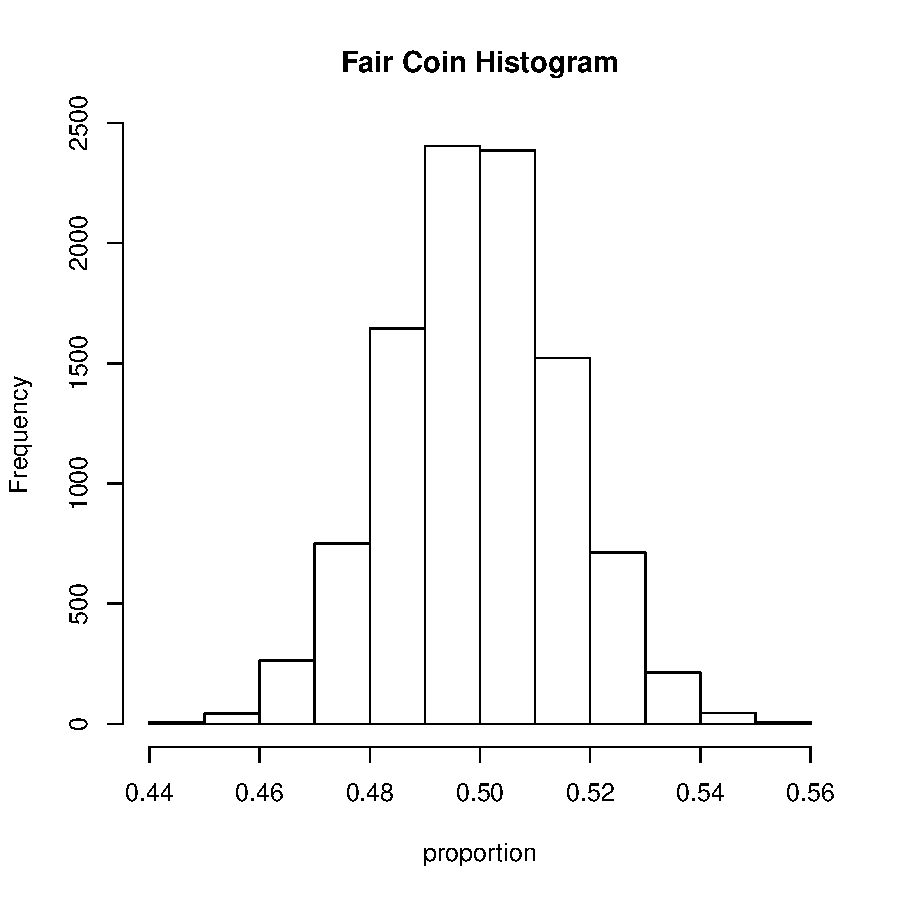
\includegraphics[width=0.6\textwidth]{figure/hist1}
\end{center}
\end{frame}
%-------------------------------------------------------------------------------


%-------------------------------------------------------------------------------
\begin{frame}
\frametitle{Say we observe...}
$\widehat{p} = \frac{501}{1000}$
\begin{center}
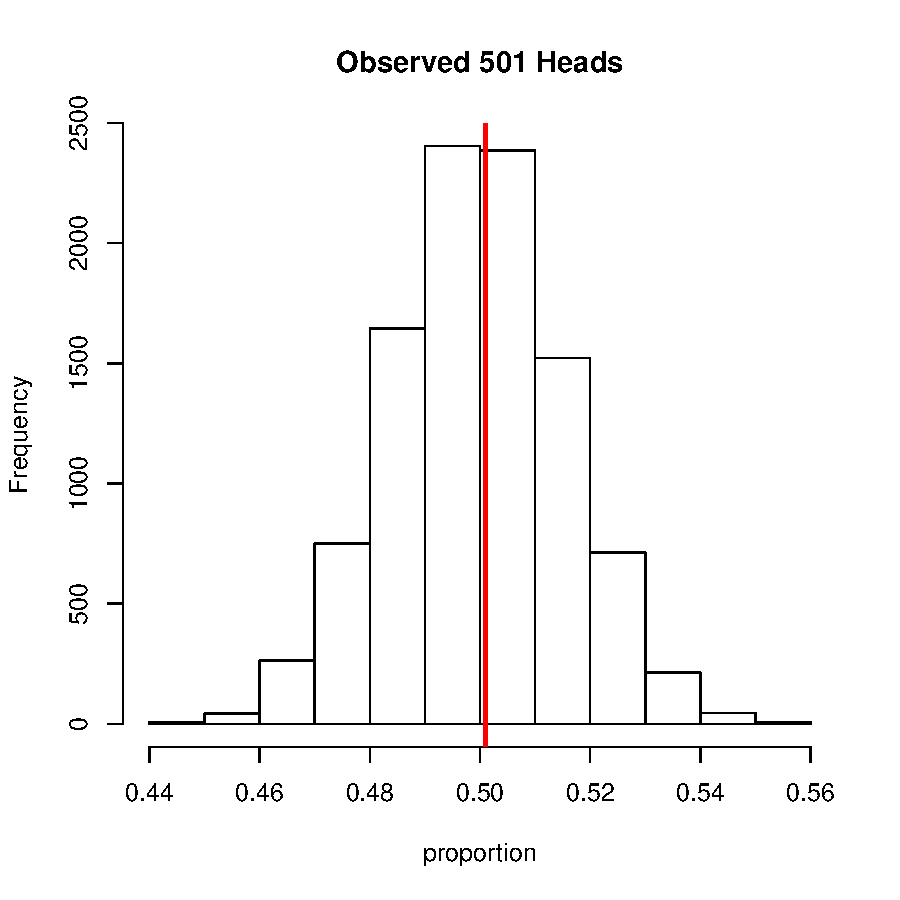
\includegraphics[width=0.6\textwidth]{figure/hist2}
\end{center}
\end{frame}
%-------------------------------------------------------------------------------


%-------------------------------------------------------------------------------
\begin{frame}
\frametitle{Say we observe...}
$\widehat{p} = \frac{525}{1000}$
\begin{center}
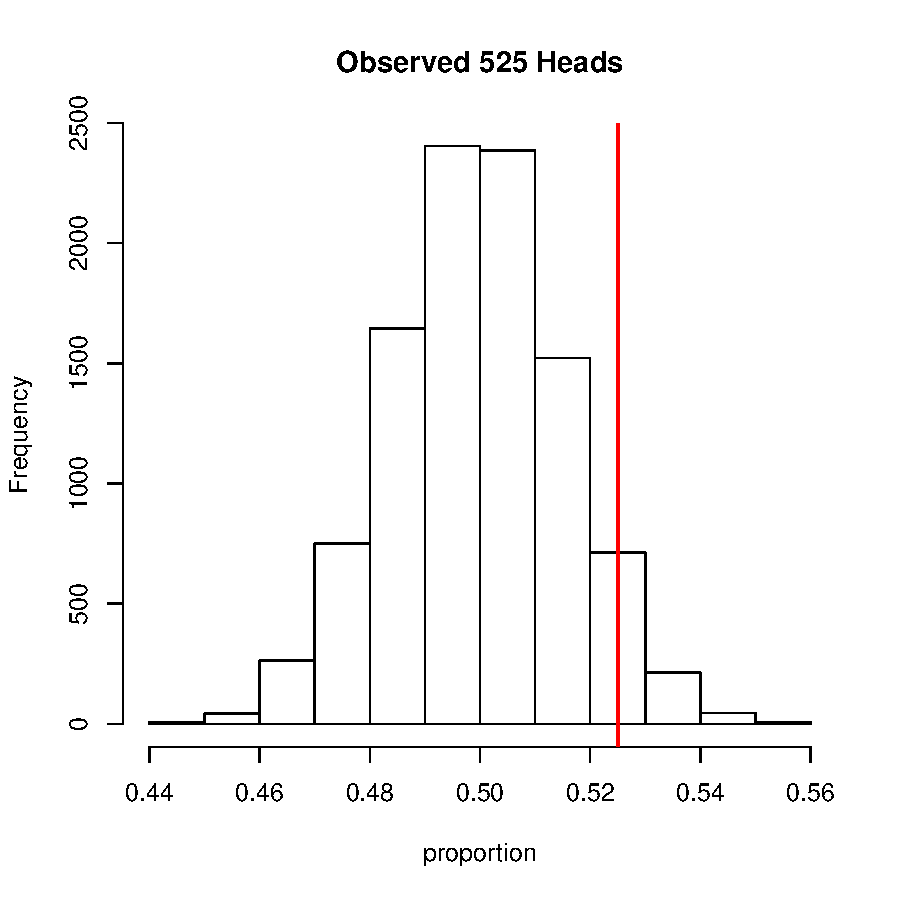
\includegraphics[width=0.6\textwidth]{figure/hist3}
\end{center}
\end{frame}
%-------------------------------------------------------------------------------


%-------------------------------------------------------------------------------
\begin{frame}
\frametitle{Say we observe...}
$\widehat{p} = \frac{900}{1000}$
\begin{center}
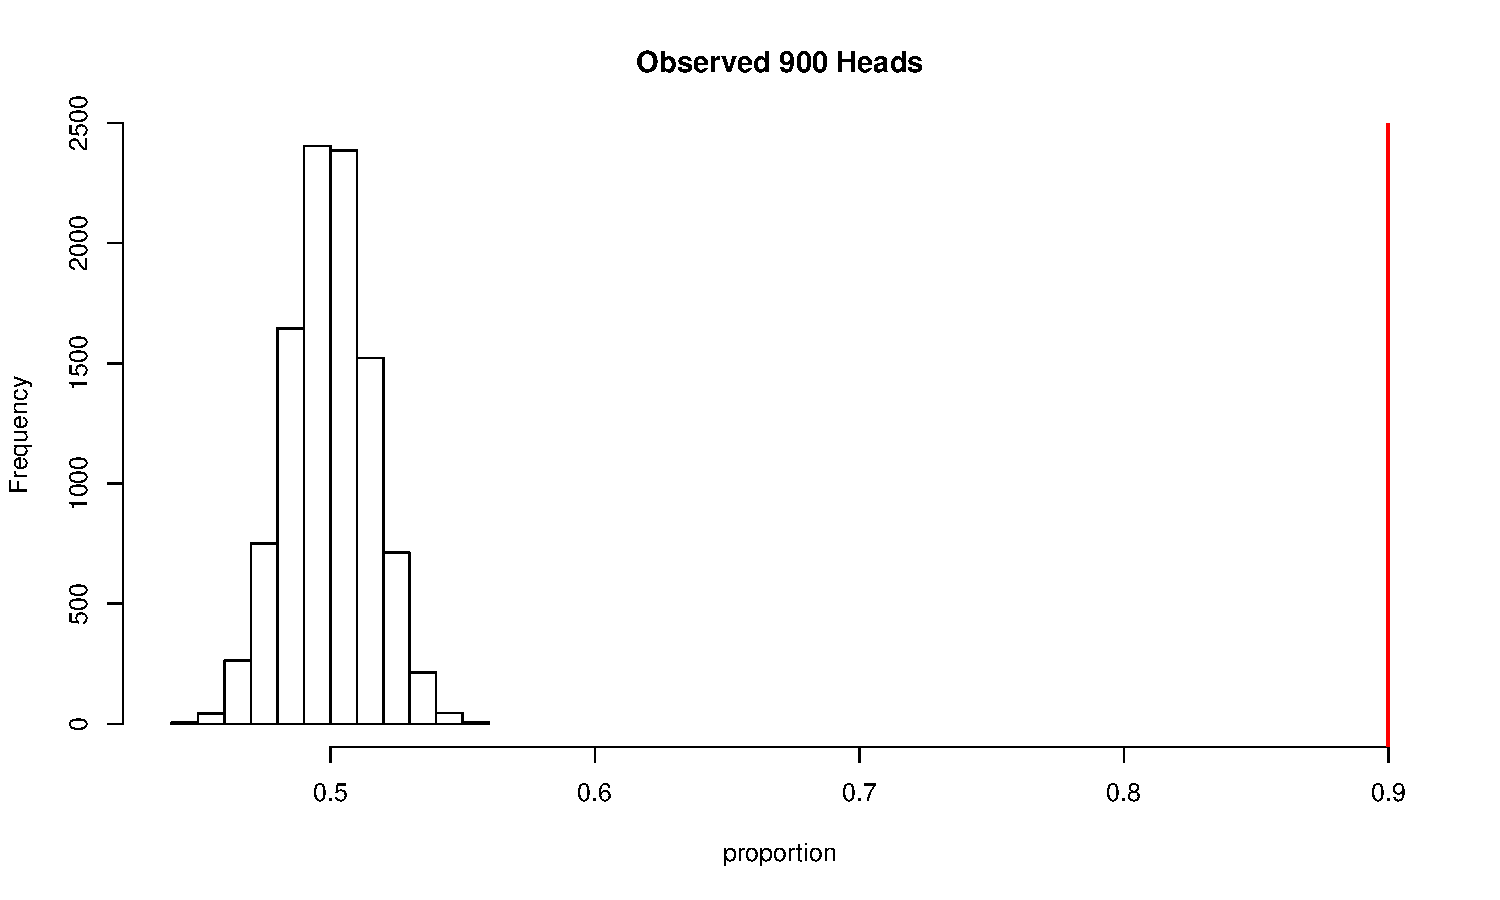
\includegraphics[width=\textwidth]{figure/hist4}
\end{center}
\end{frame}
%-------------------------------------------------------------------------------


%-------------------------------------------------------------------------------
\begin{frame}
\frametitle{Example about Sleep Habits}
A US-wide poll found that college students sleep about 7 hours a night. You suspect that Midd Kids sleep more and investigate this claim at a pre-specified $\alpha=0.01$ level.  

\vspace{0.5cm}

\pause You sample $n=110$ Midd Kids and find that $\xbar = 7.42$ and $s=1.75$ with a histogram that looks like:

\begin{center}
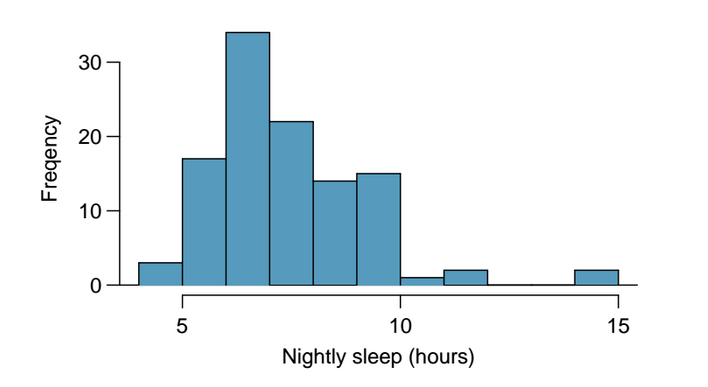
\includegraphics[width=0.6\textwidth]{figure/sleep.png}
\end{center}

\end{frame}
%-------------------------------------------------------------------------------


%-------------------------------------------------------------------------------
\begin{frame}
\frametitle{Example about Sleep Habits}

%
% Comment this
%
%\vspace{0.5cm}
%
%Let $\mu = $ \blue{true population mean} \# of hours Midd Kids sleep a night.  Then $\mu_0=7$ and: 
%\begin{itemize}
%\item $H_0: \mu = \mu_0= 7$
%\item $H_A: \mu > 7$
%\end{itemize}

\end{frame}
%-------------------------------------------------------------------------------


%-------------------------------------------------------------------------------
%\begin{frame}
%\frametitle{Example about Sleep Habits}
%
%
%%
%% Comment this
%%
%We check the 3 conditions to use the Normal model:
%\begin{enumerate}
%\pause \item Independence: $n=110 \leq$ 10\% of 2,400 (Middlebury enrollment)
%\pause \item $n \geq 30$
%\pause \item The distribution of the $n=110$ observations (Figure 4.14) is not too skewed.
%\end{enumerate}
%
%If $H_0$ is true, then $\xbar$ has mean $\mu_0$.  So in our case for $\xbar$
%\[
%z = \frac{\xbar - \mbox{null value}}{SE} = \frac{7.42 - 7}{\frac{1.75}{\sqrt{110}}} = 2.47
%\]
%
%\end{frame}
%-------------------------------------------------------------------------------


%-------------------------------------------------------------------------------
%\begin{frame}
%\frametitle{Example about Sleep Habits}
%
%%
%% Comment this
%%
%In our case, since $H_A: \mu > 7$, \blue{more extreme} means \blue{to the right} of $z=2.47$.  
%
%\vspace{0.5cm}
%
%If $H_0$ is true, then the \blue{null distribution} looks like this:  
%
%\begin{center}
%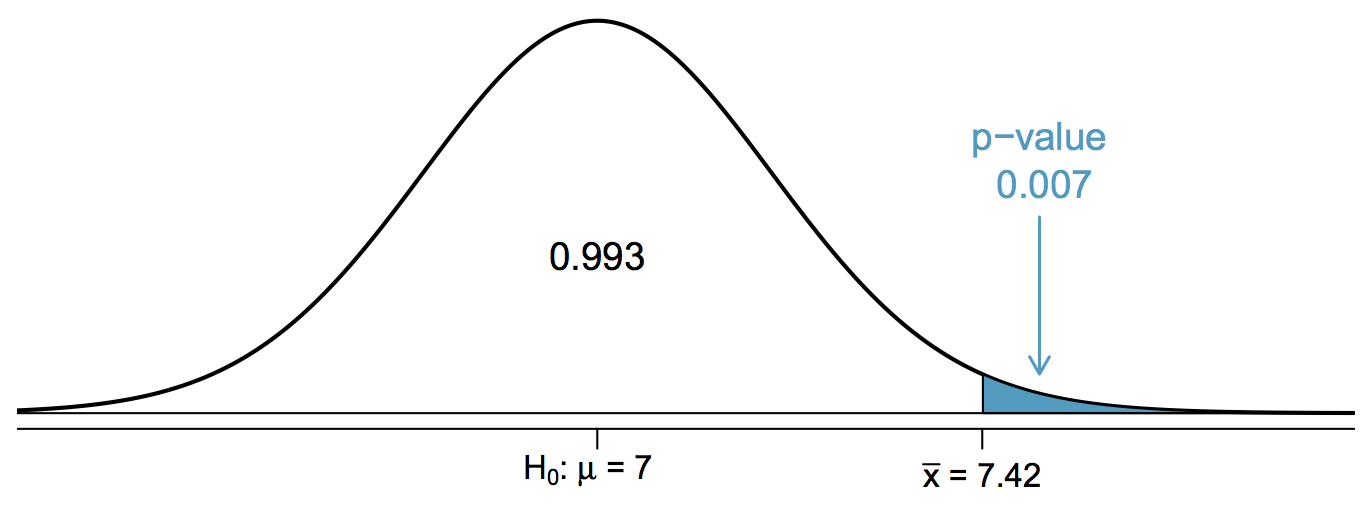
\includegraphics[width=\textwidth]{figure/pvalue.png}
%\end{center}
%
%Hence, the p-value is 0.007.
%\end{frame}
%-------------------------------------------------------------------------------


%-------------------------------------------------------------------------------
%\begin{frame}
%\frametitle{Example about Sleep Habits}
%Since the p-value $0.007 < 0.01=\alpha$, the pre-specified significance level, it has a high degree of extremeness, and thus we reject $H_0$.
%
%\end{frame}
%-------------------------------------------------------------------------------


%-------------------------------------------------------------------------------
\begin{frame}
\frametitle{Example about Sleep Habits}

\blue{Conclusion}: we reject at the $\alpha=0.01$ significance level the hypothesis that the average \# of hours Midd Kids sleep is 7, in favor of the hypothesis that they sleep more.  

\vspace{0.5cm}

\pause\blue{Correct interpretation of the p-value}:  If the null hypothesis is true ($\mu=7$), the probability of observing a sample mean $\xbar=7.42$ or greater is 0.007 (small).  

\vspace{0.5cm}

\pause\blue{Incorrect interpretation of the p-value}:  The probability that the null hypothesis ($\mu=7$) is true is 0.007.  

\end{frame}
%-------------------------------------------------------------------------------


%------------------------------------------------------------------------------
%\begin{frame}[fragile]
%\frametitle{Next Time}
%
%\begin{itemize}
%\item How big a sample size to I need? i.e. power calculations
%\item Statistical vs practical significance
%\end{itemize}
%
%\end{frame}
%------------------------------------------------------------------------------


\end{document}










%
% Laying this out now makes the procedure too formulaic
%
%%-------------------------------------------------------------------------------
%\begin{frame}
%\frametitle{In General:  Hypothesis Testing Procedure}\label{ht}
%\begin{enumerate}
%\pause\item Construct your hypothesis testing framework:
%\begin{itemize}
%\item Define $H_0$, $H_A$ and if applicable a null value.
%\item Set your significance level $\alpha$
%\end{itemize}
%\pause\item Verify that the conditions hold
%\pause\item Compute your \blue{test statistic}
%\pause\item Compute the p-value
%\begin{itemize}
%\item Identify the appropriate distribution to compare the test statistic to
%\item Depending on $H_A$, determine what constitutes being \blue{more extreme} and compute the p-value using the appropriate probability table.
%\end{itemize}
%\pause\item If the p-value is $< \alpha$, reject $H_0$.  Otherwise do not.
%\end{enumerate}
%
%\end{frame}
%%-------------------------------------------------------------------------------









